\documentclass[12pt]{article}
\usepackage[utf8]{inputenc}
\usepackage{amsmath, amssymb, amsthm}
\usepackage{enumitem}
\usepackage{geometry}
\usepackage{fancyhdr}
\usepackage{pgfplots}
\usepackage{tikz}
\usepackage{float}
\usepackage{graphicx}
\DeclareMathOperator{\Tr}{Tr}
\DeclareMathOperator{\RR}{\mathbb{R}}
\DeclareMathOperator{\rng}{rng}

% Page setup
\setlength{\headheight}{15pt}
\geometry{letterpaper, margin=1in}
\setlength{\parindent}{0pt}
\setlength{\parskip}{1em}
\pagestyle{fancy}
\fancyhf{}
\fancyhead[L]{\textbf{Sebastian Griego}}  % Replace with your name
\fancyhead[C]{\textbf{ODEs}}  % Replace with your course name
\fancyhead[R]{\textbf{Assignment \#4}}  % Replace with your assignment number
\fancyfoot[C]{\thepage}

\newenvironment{problem}[1]{
    \textbf{Problem #1:}
}{
    \rmfamily \vspace{1em}
}

\newenvironment{solution}{
    \textbf{Solution:}
    
}{
    
    \vspace{2em}
}

\begin{document}

\title{Homework \#4}  % Replace with the homework number
\author{Sebastian Griego}  % Replace with your name
\maketitle

I put all my phase planes at the end of the document.

\begin{problem}{1}
    Find the general solution to
    \[
        \frac{d\vec{x}}{dt} = \begin{pmatrix} 1 & 0 \\ 0 & a \end{pmatrix} \vec{x}
    \]
    Plot the phase diagram for \(a = \pm 1\). What happens when \(a = 0\)?
\end{problem}

\begin{solution}
    Clearly, the eigenvalues of this matrix are \(\lambda_1 = 1\) and \(\lambda_2 = a\), and the eigenvectors are \(\vec{v}_1 = \begin{pmatrix} 1 \\ 0 \end{pmatrix}\) and \(\vec{v}_2 = \begin{pmatrix} 0 \\ 1 \end{pmatrix}\). Thus, the general solution to this system is given by
    \[
        \begin{aligned}
            \vec{x}(t) &= V \begin{pmatrix} e^{\lambda_1 t} & 0 \\ 0 & e^{\lambda_2 t} \end{pmatrix} V^{-1} \vec{x}(0) \\
            &= \begin{pmatrix} 1 & 0 \\ 0 & 1 \end{pmatrix} \begin{pmatrix} e^{t} & 0 \\ 0 & e^{at} \end{pmatrix} \begin{pmatrix} 1 & 0 \\ 0 & 1 \end{pmatrix} \vec{x}(0) \\
            &= \begin{pmatrix} e^{t} & 0 \\ 0 & e^{at} \end{pmatrix} \vec{x}(0) \\
            &= x_1(0)e^t + x_2(0)e^{at}.
        \end{aligned}
    \]

    When \(a = 1\), the solution is
    \[
        \vec{x}(t) = x_1(0)e^t + x_2(0)e^t = (x_1(0) + x_2(0))e^t.
    \]
    A source.

    When \(a = -1\), the solution is
    \[
        \vec{x}(t) = x_1(0)e^t + x_2(0)e^{-t}.
    \]
    A saddle.

    When \(a = 0\), the solution is
    \[
        \begin{aligned}
            \vec{x}(t) &= x_1(0)e^t + x_2(0)e^{0t} \\
            &= x_1(0)e^t + x_2(0).
        \end{aligned}
    \]
    A source.

    Phase planes at the end of the document.
    
    
\end{solution}

\newpage

\begin{problem}{2}
    Write
    \[
        \ddot{x} + \dot{x} + 4x = 0
    \]
    as a system, find its general solution, and sketch its phase diagram.
\end{problem}

\begin{solution}
    Let \(y = \frac{dx}{dt}\). Then, the equation becomes
    \[
        \frac{dy}{dt} + y + 4x = 0 \\
    \]
    This gives the system
    \[
        \begin{aligned} 
            \frac{dy}{dt} &= -y - 4x \\
            \frac{dx}{dt} &= y
        \end{aligned}
    \]
    Write as a matrix equation
    \[
        \frac{d}{dt} \begin{pmatrix} x \\ y \end{pmatrix} = \begin{pmatrix} 0 & 1 \\ -4 & -1 \end{pmatrix} \begin{pmatrix} x \\ y \end{pmatrix}
    \]
    Eigenvalues:
    \[
        \begin{aligned}
            \lambda &= \frac{1}{2}(\Tr(A) \pm \sqrt{\Tr(A)^2 - 4\det(A)}) \\
            &= \frac{1}{2}(-1 \pm \sqrt{1 - 16}) \\
            &= \frac{1}{2}(-1 \pm i\sqrt{15}) \\
        \end{aligned}
    \]
    Eigenvectors:
    \[
        \begin{aligned}
            A - \lambda I &= \begin{pmatrix} 0 & 1 \\ -4 & -1 \end{pmatrix} - \begin{pmatrix} \frac{1}{2}(-1 + i\sqrt{15}) & 0 \\ 0 & \frac{1}{2}(-1 + i\sqrt{15}) \end{pmatrix} \\
            &= \begin{pmatrix} \frac{1}{2} - \frac{i\sqrt{15}}{2} & 1 \\ -4 & \frac{-1}{2} - \frac{i\sqrt{15}}{2} \end{pmatrix}
        \end{aligned}
    \]
    Solving for the eigenvector, we get
    \[
        \begin{pmatrix} \frac{1}{2} - \frac{i\sqrt{15}}{2} & 1 \\ -4 & \frac{-1}{2} - \frac{i\sqrt{15}}{2} \end{pmatrix} \begin{pmatrix} v_1 \\ v_2 \end{pmatrix} = \begin{pmatrix} 0 \\ 0 \end{pmatrix}
    \]
    Gives
    \[
        -4v_1 + \left(\frac{-1}{2} - \frac{i\sqrt{15}}{2}\right)v_2 = 0
    \]
    Let \(v_2 = 1\). Then,
    \[
        -4v_1 + \left(\frac{-1}{2} - \frac{i\sqrt{15}}{2}\right) = 0 \implies v_1 = \frac{-1}{8} - \frac{i\sqrt{15}}{8}
    \]
    Thus, the eigenvector is
    \[
        \vec{v}_1 = \begin{pmatrix} \frac{-1}{8} - \frac{i\sqrt{15}}{8} \\ 1 \end{pmatrix}
    \]
    Second eigenvector:
    \[
        \begin{pmatrix} \frac{1}{2} + \frac{i\sqrt{15}}{2} & 1 \\ -4 & \frac{-1}{2} + \frac{i\sqrt{15}}{2} \end{pmatrix} \begin{pmatrix} v_1 \\ v_2 \end{pmatrix} = \begin{pmatrix} 0 \\ 0 \end{pmatrix}
    \]
    Gives
    \[
        -4v_1 + \left(\frac{-1}{2} + \frac{i\sqrt{15}}{2}\right)v_2 = 0
    \]
    Let \(v_2 = 1\). Then,
    \[
        -4v_1 + \left(\frac{-1}{2} + \frac{i\sqrt{15}}{2}\right) = 0 \implies v_1 = \frac{-1}{8} + \frac{i\sqrt{15}}{8}
    \]
    Thus, the eigenvector is
    \[
        \vec{v}_2 = \begin{pmatrix} \frac{-1}{8} + \frac{i\sqrt{15}}{8} \\ 1 \end{pmatrix}
    \]
    Define \(V\) and \(V^{-1}\) as follows:
    \[
        \begin{aligned}
            V &= \begin{pmatrix} \frac{-1}{8} - \frac{i\sqrt{15}}{8} & \frac{-1}{8} + \frac{i\sqrt{15}}{8} \\ 1 & 1 \end{pmatrix} \\
            V^{-1} &= \frac{1}{\frac{i\sqrt{15}}{4}}\begin{pmatrix} 1 & \frac{1}{8} - \frac{i\sqrt{15}}{8} \\ -1 & \frac{-1}{8} - \frac{i\sqrt{15}}{8} \end{pmatrix}
        \end{aligned}
    \]
    Then, the general solution is given by
    \[
        \vec{x}(t) = \begin{pmatrix} \frac{-1}{8} - \frac{i\sqrt{15}}{8} & \frac{-1}{8} + \frac{i\sqrt{15}}{8} \\ 1 & 1 \end{pmatrix}\begin{pmatrix} e^{\left(\frac{-1}{2} + \frac{i\sqrt{15}}{2}\right)t} & 0 \\ 0 & e^{\left(\frac{-1}{2} - \frac{i\sqrt{15}}{2}\right)t} \end{pmatrix} \frac{1}{\frac{i\sqrt{15}}{4}}\begin{pmatrix} 1 & \frac{1}{8} - \frac{i\sqrt{15}}{8} \\ -1 & \frac{-1}{8} - \frac{i\sqrt{15}}{8} \end{pmatrix} \vec{x}_0
    \]
\end{solution}

\newpage

\begin{problem}{3}
    Write
    \[
        \ddot{x} + 4x = 0
    \]
    as a system, find its general solution, and sketch its phase diagram.
\end{problem}

\begin{solution}
    Let \(y = \frac{dx}{dt}\). Then, the equation becomes
    \[
        \frac{dy}{dt} + 4x = 0
    \]
    This gives the system
    \[
        \begin{aligned} 
            \frac{dy}{dt} &= -4x \\
            \frac{dx}{dt} &= y
        \end{aligned}
    \]
    Write as a matrix equation
    \[
        \frac{d}{dt} \begin{pmatrix} x \\ y \end{pmatrix} = \begin{pmatrix} 0 & 1 \\ -4 & 0 \end{pmatrix} \begin{pmatrix} x \\ y \end{pmatrix}
    \]
    Eigenvalues:
    \[
        \begin{aligned}
            \lambda &= \frac{1}{2}(\Tr(A) \pm \sqrt{\Tr(A)^2 - 4\det(A)}) \\
            &= \frac{1}{2}(0 \pm \sqrt{0 - 16}) \\
            &= \pm 2i
        \end{aligned}
    \]
    Eigenvectors:
    \[
        \begin{pmatrix} -2i & 1 \\ -4 & -2i \end{pmatrix} \begin{pmatrix} v_1 \\ v_2 \end{pmatrix} = \begin{pmatrix} 0 \\ 0 \end{pmatrix}
    \]
    Gives
    \[
        -2iv_1 + v_2 = 0 \implies v_2 = 2iv_1
    \]
    Let \(v_1 = -i\). Then,
    \[
        v_2 = 2i(-i) = 2
    \]
    Thus, the eigenvector is
    \[
        \vec{v}_1 = \begin{pmatrix} -i \\ 2 \end{pmatrix}
    \]
    Second eigenvector:
    \[
        \begin{pmatrix} 2i & 1 \\ -4 & 2i \end{pmatrix} \begin{pmatrix} v_1 \\ v_2 \end{pmatrix} = \begin{pmatrix} 0 \\ 0 \end{pmatrix}
    \]
    Gives
    \[
        2iv_1 + v_2 = 0 \implies v_2 = -2iv_1
    \]
    Let \(v_1 = i\). Then,
    \[
        v_2 = -2i(i) = 2
    \]
    Thus, the eigenvector is
    \[
        \vec{v}_2 = \begin{pmatrix} i \\ 2 \end{pmatrix}
    \]
    Define \(V\) and \(V^{-1}\) as follows:
    \[
        \begin{aligned}
            V &= \begin{pmatrix} -i & i \\ 2 & 2 \end{pmatrix} \\
            V^{-1} &= \frac{i}{4}\begin{pmatrix} 2 & -i \\ -2 & -i \end{pmatrix}
        \end{aligned}
    \]
    Then, the general solution is given by
    \[
        \vec{x}(t) = \begin{pmatrix} -i & i \\ 2 & 2 \end{pmatrix} \begin{pmatrix} e^{\left(2i\right)t} & 0 \\ 0 & e^{\left(-2i\right)t} \end{pmatrix} \frac{i}{4}\begin{pmatrix} 2 & -i \\ -2 & -i \end{pmatrix} \vec{x}_0
    \]
\end{solution}

\newpage

\begin{problem}{4}
    Let the \(2 \times 2\) matrix \(A\) have real, distinct eigenvalues \(\lambda\) and \(\mu\). Suppose
that an eigenvector of \(\lambda\) is \((1, 0)^T\) and an eigenvector of \(\mu\) is \((-1, 1)^T\).
Sketch the phase portraits of \(\dot{\vec{x}} = A\vec{x}\) for the following cases:

(a) \(0 < \lambda < \mu\), (b) \(0 < \mu < \lambda\), (c) \(\lambda < \mu < 0\),\\
(d) \(\lambda < 0 < \mu\), (e) \(\mu < 0 < \lambda\), (f) \(\lambda = 0\), \(\mu > 0\).

\end{problem}

\begin{solution}
    \begin{figure}[H]
        \centering
        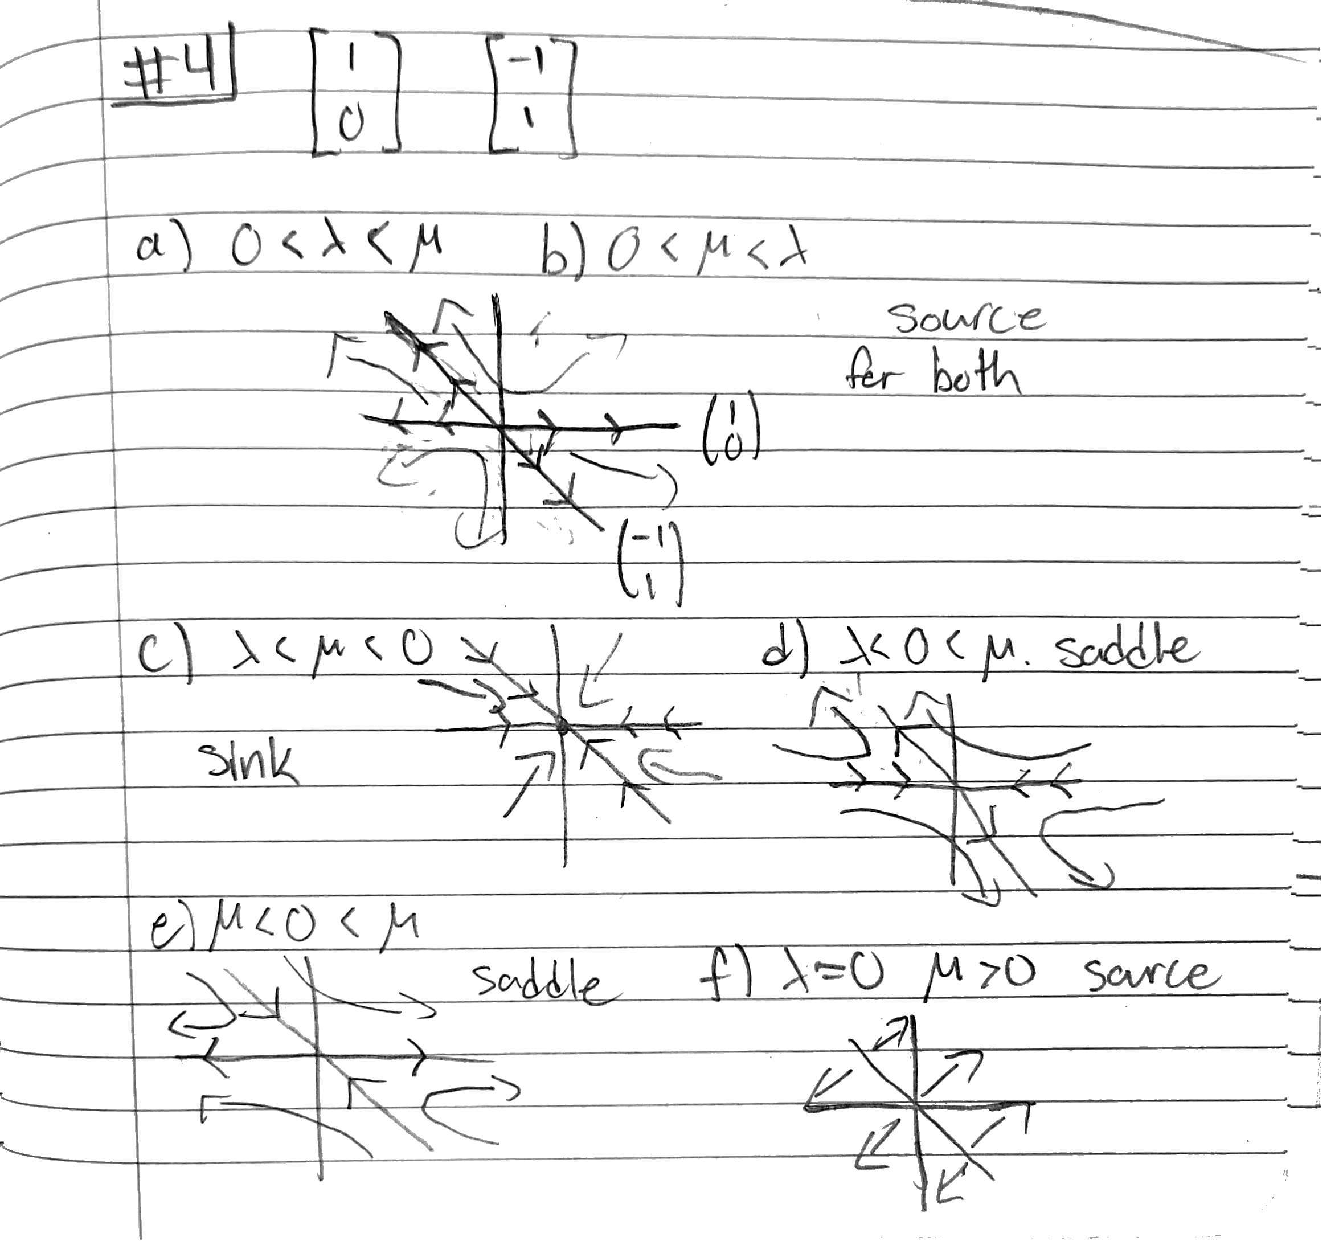
\includegraphics[width=0.6\textwidth]{4.pdf}
    \end{figure}
\end{solution}

\newpage

\begin{problem}{5}
    Find the general solution to
    \[
        \frac{d\vec{x}}{dt} = \begin{pmatrix} 3 & -2 \\ 1 & 1 \end{pmatrix}\vec{x}
    \]
    Plot the phase diagram.
\end{problem}

\begin{solution}
    Eigenvalues:
    \[
        \begin{aligned}
            \lambda &= \frac{1}{2}(\Tr(A) \pm \sqrt{\Tr(A)^2 - 4\det(A)}) \\
            &= \frac{1}{2}(4 \pm \sqrt{16 - 20}) \\
            &= 2 \pm i
        \end{aligned}
    \]
    Eigenvectors:
    \[
        \begin{pmatrix} 1 - i & -2 \\ 1 & -1-i \end{pmatrix} \begin{pmatrix} v_1 \\ v_2 \end{pmatrix} = \begin{pmatrix} 0 \\ 0 \end{pmatrix}
    \]
    Gives
    \[
        v_1 - (1 + i)v_2 = 0 \implies v_1 = (1 + i)v_2
    \]
    Let \(v_2 = 1\). Then,
    \[
        v_1 = 1 + i
    \]
    Thus, the eigenvector is
    \[
        \vec{v}_1 = \begin{pmatrix} 1 + i \\ 1 \end{pmatrix}
    \]

    Second eigenvector:
    \[
        \begin{pmatrix} 1 + i & -2 \\ 1 & -1+i \end{pmatrix} \begin{pmatrix} v_1 \\ v_2 \end{pmatrix} = \begin{pmatrix} 0 \\ 0 \end{pmatrix}
    \]
    Gives
    \[
        v_1 + (-1 + i)v_2 = 0 \implies v_1 = (1 - i)v_2
    \]
    Let \(v_2 = 1\). Then,
    \[
        v_1 = 1 - i
    \]
    Thus, the eigenvector is
    \[
        \vec{v}_2 = \begin{pmatrix} 1 - i \\ 1 \end{pmatrix}
    \]
    Define \(V\) and \(V^{-1}\) as follows:
    \[
        \begin{aligned}
            V &= \begin{pmatrix} 1 + i & 1 - i \\ 1 & 1 \end{pmatrix} \\
            V^{-1} &= \frac{1}{2i}\begin{pmatrix} 1 & -1 + i \\ -1 & 1 + i \end{pmatrix}
        \end{aligned}
    \]
    Then, the general solution is given by
    \[
        \vec{x}(t) = \begin{pmatrix} 1 + i & 1 - i \\ 1 & 1 \end{pmatrix} \begin{pmatrix} e^{(2+i)t} & 0 \\ 0 & e^{(2-i)t} \end{pmatrix} \frac{1}{2i}\begin{pmatrix} 1 & -1 + i \\ -1 & 1 + i \end{pmatrix} \vec{x}_0
    \]
\end{solution}

\newpage

\begin{problem}{6}
    Find the solution to
    \[
        \frac{d\vec{x}}{dt} = \begin{pmatrix} 2 & 1 \\ 1 & 2 \end{pmatrix}\vec{x} + \begin{pmatrix} t \\ 1 \end{pmatrix} \;,\;\vec{x}(0) = \begin{pmatrix} 1 \\ 0 \end{pmatrix}
    \]
\end{problem}

\begin{solution}
    Find the eigenvalues:
    \[
        \begin{aligned}
            \lambda &= \frac{1}{2}(\Tr(A) \pm \sqrt{\Tr(A)^2 - 4\det(A)}) \\
            &= \frac{1}{2}(4 \pm \sqrt{4^2 - 4 \cdot 3})\\
            &= \frac{1}{2}(4 \pm \sqrt{4})\\
            &= 2 \pm 1\\
        \end{aligned}
    \]
    \[
        \lambda_1 = 3, \lambda_2 = 1
    \]
    Eigenvectors:
    \[
        \begin{pmatrix} -1 & 1 \\ 1 & -1 \end{pmatrix} \begin{pmatrix} v_1 \\ v_2 \end{pmatrix} = \begin{pmatrix} 0 \\ 0 \end{pmatrix}
    \]
    Gives
    \[
        -v_1 + v_2 = 0 \implies v_1 = v_2
    \]
    Let \(v_1 = 1\). Then,
    \[
        v_2 = 1
    \]
    Thus, the eigenvector is
    \[
        \vec{v}_1 = \begin{pmatrix} 1 \\ 1 \end{pmatrix}
    \]
    Second eigenvector:
    \[
        \begin{pmatrix} 1 & 1 \\ 1 & 1 \end{pmatrix} \begin{pmatrix} v_1 \\ v_2 \end{pmatrix} = \begin{pmatrix} 0 \\ 0 \end{pmatrix}
    \]
    Gives
    \[
        v_1 + v_2 = 0 \implies v_1 = -v_2
    \]
    Let \(v_1 = 1\). Then,
    \[
        v_2 = -1
    \]
    Thus, the eigenvector is
    \[
        \vec{v}_2 = \begin{pmatrix} 1 \\ -1 \end{pmatrix}
    \]
    Define \(V\) and \(V^{-1}\) as follows:
    \[
        \begin{aligned}
            V &= \begin{pmatrix} 1 & 1 \\ 1 & -1 \end{pmatrix} \\
            V^{-1} &= \frac{-1}{2}\begin{pmatrix} -1 & -1 \\ -1 & 1 \end{pmatrix}
        \end{aligned}
    \]
    Then, the general solution is given by
    \[
        \vec{x}(t) = \Phi(t,0) \vec{x}_0 + \int_0^t \Phi(t,s) \vec{f}(s) ds
    \]
    where
    \[
        \Phi(t,s) = \begin{pmatrix} 1 & 1 \\ 1 & -1 \end{pmatrix} \begin{pmatrix} e^{3(t-s)} & 0 \\ 0 & e^{t-s} \end{pmatrix} \frac{-1}{2}\begin{pmatrix} -1 & -1 \\ -1 & 1 \end{pmatrix}
    \]
    and
    \[
        \vec{f}(s) = \begin{pmatrix} s \\ 1 \end{pmatrix}
    \]
    Simplify the integral
    \[
        \begin{aligned}
            \int_0^t \Phi(t,s) \vec{f}(s) ds &= \int_0^t \begin{pmatrix} 1 & 1 \\ 1 & -1 \end{pmatrix} \begin{pmatrix} e^{3(t-s)} & 0 \\ 0 & e^{t-s} \end{pmatrix} \frac{-1}{2}\begin{pmatrix} -1 & -1 \\ -1 & 1 \end{pmatrix} \begin{pmatrix} s \\ 1 \end{pmatrix} ds \\
            &= \int_0^t \begin{pmatrix} e^{3(t-s)} & e^{t-s} \\ e^{3(t-s)} & -e^{t-s} \end{pmatrix} \begin{pmatrix} \frac{1}{2} & \frac{1}{2} \\ \frac{1}{2} & -\frac{1}{2} \end{pmatrix} \begin{pmatrix} s \\ 1 \end{pmatrix} ds \\
            &= \int_0^t \begin{pmatrix} e^{3(t-s)} & e^{t-s} \\ e^{3(t-s)} & -e^{t-s} \end{pmatrix} \begin{pmatrix} \frac{s}{2} + \frac{1}{2} \\ \frac{s}{2} - \frac{1}{2} \end{pmatrix} ds \\
            &= \frac{1}{2} \int_{0}^{t} \begin{pmatrix} e^{3(t-s)} & e^{t-s} \\ e^{3(t-s)} & -e^{t-s} \end{pmatrix} \begin{pmatrix} s + 1 \\ s - 1 \end{pmatrix} ds \\
            &= \frac{1}{2} \int_{0}^{t} \begin{pmatrix} e^{3(t-s)}(s + 1) + e^{t-s}(s - 1) \\ e^{3(t-s)}(s + 1) - e^{t-s}(s - 1) \end{pmatrix} ds \\
            &= \frac{1}{2} \begin{pmatrix} \int_{0}^{t} e^{3(t-s)}(s + 1) ds + \int_{0}^{t} e^{t-s}(s - 1) ds \\ \int_{0}^{t} e^{3(t-s)}(s + 1) ds - \int_{0}^{t} e^{t-s}(s - 1) ds \end{pmatrix}\\
            &= \frac{1}{2} \begin{pmatrix} \frac{1}{9}(-3t + 4te^{3t} - 4) + \frac{1}{9}(-3t -2e^{3t}+2) \\ \frac{1}{9}(-3t + 4te^{3t} - 4) - \frac{1}{9}(-3t -2e^{3t}+2) \end{pmatrix}
        \end{aligned}
    \]
    The solution is
    \[
        \begin{aligned}
            \vec{x}(t) &= \Phi(t,0) \vec{x}_0 + \int_0^t \Phi(t,s) \vec{f}(s) ds\\
            &= \begin{pmatrix} 1 & 1 \\ 1 & -1 \end{pmatrix} \begin{pmatrix} e^{3t} & 0 \\ 0 & e^{t} \end{pmatrix} \frac{1}{2}\begin{pmatrix} -1 & -1 \\ -1 & 1 \end{pmatrix} \begin{pmatrix} 1 \\ 0 \end{pmatrix} + \frac{1}{2} \begin{pmatrix} \frac{1}{9}(-3t + 4te^{3t} - 4) + \frac{1}{9}(-3t -2e^{3t}+2) \\ \frac{1}{9}(-3t + 4te^{3t} - 4) - \frac{1}{9}(-3t -2e^{3t}+2) \end{pmatrix} \\
        \end{aligned}
    \]

\newpage

\section{Phase Planes}

\begin{figure}[H]
    \centering
    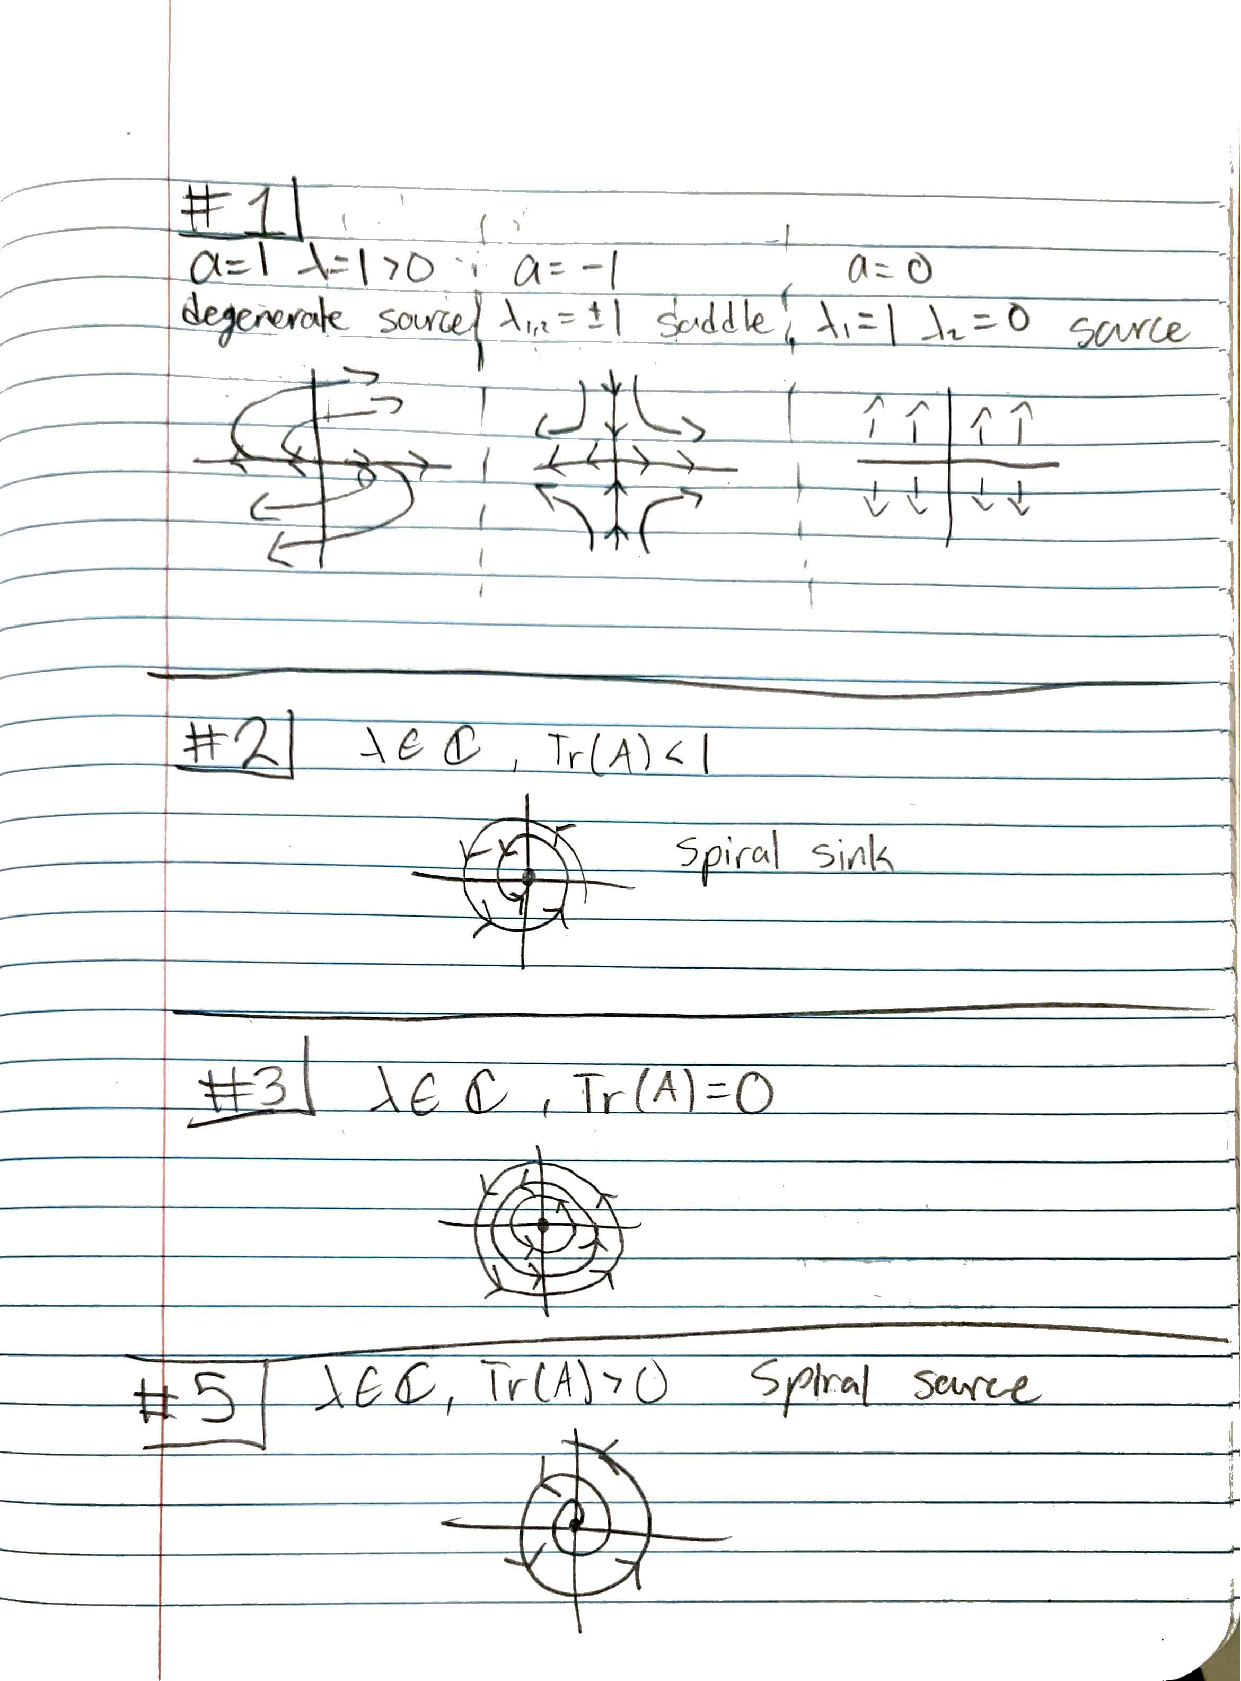
\includegraphics[width=0.6\textwidth]{123.pdf}
\end{figure}
    
    
    

\end{solution}

\end{document}